\section{Models and Counter-models for Constructive logic}


In our previous investigations of constructive validity, we have shown that certain arguments are constructively valid by demonstrating specifically how to carry out those constructions.  We have also, in some cases, shown that 
if a particular argument were constructively valid then
we could use it to prove the constructive validity of DNE and LEM, which therefore demonstrates (by \emph{modus tollens}) that the argument is \emph{not} constructively valid.
However, we have not been able to do this in all cases: in particular, we could not find a way to deduce LEM from the Third de Morgan Law.  Moreover, it is not that case that all constructively invalid arguments allow us to derive constructively unacceptable conclusions like LEM and DNE.\footnote{
Specifically, classical logic is obtained by adding LEM to constructive logic, but there are \emph{intermediate logics} between constructive and classical logic which add new axioms that cannot be proved constructively but which are not as powerful as classical logic. 
}

We therefore need more powerful techniques.  In this Section we will investigate a few different approaches to demonstrating the constructive validity or invalidity of arguments, and see how they are related to one another.

%\newpage
\subsection{Truth tables and tautologies}
\label{sec:Models-TruthTables}

A standard way of establishing the validity of a formula in classical propositional logic (i.e. an expression built up from $\AND$, $\OR$, $\NOT$, $\IMPLIES$, and variables representing propositions)
is by constructing a \emph{truth table}.  Each propositional variable can be either true or false, and so for a formula involving $n$ variables there are $2^n$ possible assignments of truth values to its variables.  We can therefore work out the truth value of the formula itself under each possible assignment.  If the formula is true for every posible assignment of truth values then it is a \emph{tautology} of classical propositional logic.  A further result then shows that a formula can be proved in CPL if and only if it is a tautology.

For example, consider the third de Morgan law (or rather, the formula we get from it by applying the Deduction theorem)
\[
\NOT (P \AND Q) \IMPLIES ((\NOT P) \OR (\NOT Q))
\]
There are two propositional variables, so we have $2^2$ possible assignments of truth values to them.  In each case we can work out the truth value of the formula:\\
\begin{table}[h]
\centering
\begin{tabular}{c c|c c c}
P &	Q & $\NOT(P \AND Q)$ &	$(\NOT P) \OR (\NOT Q)$ &	$\NOT (P \AND Q) \IMPLIES ((\NOT P) \OR (\NOT Q))$ \\
\hline
T & T & F & F & T\\
T & F & T & T & T\\
F & T & T & T & T\\
F & F & T & T & T\\
\end{tabular}
\end{table}\\
The formula is true under any assignment, and so it is a classical tautology.

This procedure has the advantage that it is guaranteed either to  confirm that a formula is a tautology or to provide a \emph{counterexample} -- a particular assignment of truth values to variables under which the formula is false.  Moreover this procedure is entirely mechanical, and so a computer can check the validity of any finite formula of CPL.  Finally, if we are given a putative counterexample we can immediately verify it for ourselves by evaluating the formula with those values.  We therefore don't simply have to trust the computer program when it tells us that a formula is not a tautology.

These features are exactly what we want for our system: invalid arguments can be identified \emph{automatically}, and their invalidity is certified by a \emph{witness}, i.e. the particular counterexample.  It would therefore be useful to be able to adapt this method from classical to constructive logic.


\subsection{Boolean and Heyting algebras}

The modification of this technique that's required is conceptually simple.  The truth values we use in classical logic, $T$ and $F$, form a \terminology{Boolean algebra} -- a collection of values on which we can define the operations $\AND$, $\OR$, $\NOT$, and $\IMPLIES$, all of which behave as we expect, and which satisfies $\NOT \NOT x = x$ for all elements.  We can build up the definition of a Boolean algebra in stages.  

A \terminology{lattice} is a set of elements equipped with a preordering -- a relationship $\leq$ that is reflexive and transitive -- such that any pair of elements has both a greatest lower bound and a least upper bound.  We write the greatest lower bound of $x$ and $y$ as $x \glb y$, and the least upper bound as $x \lub y$.

A lattice is \terminology{distributive} if for all $x, y, z$ in the lattice we have
\[
x \glb (y \lub z) = (x \glb y) \lub (x \glb z)
\]
or, equivalently,
\[
x \lub (y \glb z) = (x \lub y) \glb (x \lub z)
\]
%or equivalently,
%\[
%x\wedge z = y\wedge z 
%\;\mbox{  and  }\;
% x\vee z = y\vee z 
%\;\mbox{  implies  } \;
%x=y
%\]
This allows us to give a particularly simple representation of any finite distributive lattice: we can represent it as a collection of (some of the) subsets of some finite set $S$.  The ordering relation is then given by subset inclusion, while $\glb$ and $\lub$ are given by intersection and union respectively.\footnote{This representation theorem was proved by Birkhoff (1937).
}  We can therefore use $\glb$ and $\lub$ to represent conjunction and disjunction in logic: the items in $x \glb y$ are those in both $x$ and $y$, while the items in $x \lub y$ are those in either $x$ or $y$.

A lattice is \terminology{bounded} if it has elements $1$ and $0$ such that for all elements $x$ in the lattice, $0 \leq x \leq 1$.  It is easy to confirm that $x \lub 0 = x = x \glb 1$, $x \glb 0 = 0$, and $x \lub 1 = 1$.  Every finite distributive lattice is bounded, with $S$ as $1$ and $\varnothing$ as $0$.

How do we represent implication, $x \IMPLIES y$?  Given a distributive lattice, we can consider for any $x$ and $y$ the elements $z$ such that $x \glb z \leq y$.  In the representation as subsets, these are the sets disjoint from $x \setminus y$
(where $x \setminus y$ is the set of items in $x$ but not in $y$).  That is, if an item is in such a $z$ and also in $x$, then it must be in $y$ as well.  If there is a \emph{maximal} such $z$ for a given $x$ and $y$ then we take this element to represent $x \IMPLIES y$.  

A \terminology{Heyting algebra} is a bounded distributive lattice in which for every pair $x$, $y$ there is an element 
\[
x \to y \DefinedAs \mbox{max}\setSuchThat{z}{x \glb z \leq y}
\]
In particular, in a finite distributive lattice such a maximum always exists, since the union of all such $z$ is an element of the lattice, and so every finite distributive lattice is a Heyting algebra.

In any Heyting algebra we can define $\NOT x$ as $x \to 0$ (in accordance with our definition in our constructive logic).  In the representation as subsets this is the largest subset in the lattice that is \emph{disjoint} with $x$ -- that is, it's some subset of $S \setminus x$.  However, in an arbitrary Heyting algebra $S \setminus x$ itself will not in general be an element of the lattice whenever $x$ is, and so $\NOT x$ will in general be some \emph{proper} subset of $S \setminus x$.  Hence $\NOT \NOT x$ will not in general be equal to $x$.

Heyting algebras therefore provide a mathematical structure in which we can do logic without imposing $\NOT \NOT x = x$.  However, nothing in our definition \emph{prevents} $\NOT \NOT x$ from being equal to $x$ for any given element.  A Heyting algebra in which this equality does in fact hold for every element is a \terminology{Boolean algebra}.  A Heyting algebra that is \emph{not} Boolean is called a \emph{proper} Heyting algebra.  In general in a proper Heyting algebra we may have some elements satisfying $\NOT \NOT x = x$, but of course we must have at least one that does not satisfy this equality.




\subsection{Examples of Heyting algebras}

To specify a Heyting algebra we only need to give the preordering relation between its elements, since all the logical operations are defined in terms of this ordering.  We can therefore present a finite Heyting algebra visually by means of its \emph{Hasse diagram}; to draw this, we draw a dot for each element, arrange the dots so that greater elements are above lesser ones, and connect dots $x$ and $z$ by a line iff one element \emph{covers} the other (i.e. $x \leq z$ and there is no element $y$ such that $x \leq y \leq z$).  The information presented in the Hasse diagram is sufficient to reconstruct the entire preordering relation, and therefore the Heyting algebra.

Alternatively, it is also sufficient to specify the truth table for $\to$, because from this truth table we can reconstruct the preordering relation:
\begin{Lemma}
$x \leq y$ if and only if $x \to y = 1$.
\end{Lemma}
\begin{Proof}
We use the subset representation of the finite Heyting algebra, in which the above becomes
$x \subseteq y$ if and only if $x \to y = S$.
If $x \to y = S$ then by the definition of $\to$ we have $x = x \intersect S  \subseteq y$.  Conversely if $x \subseteq y$ then $S$ satisfies this relation, and is of course the greatest element satisfying this relation, so $x \to y = S$.
\end{Proof}
Figure \ref{fig:3HeytingAlgebras} shows the Hasse diagrams of three Heyting algebras, whose truth tables are given in Table \ref{tab:3HeytingAlgebras}.

\begin{table}[h]
\centering
\begin{tabular}{c|ccccc}
$\to$	& 0 & a & b & 1 \\
\hline
0	&	1 & 1 & 1 & 1	\\
a	&	b & 1 & b & 1 	\\
b	&	a & a & 1 & 1 	\\
1	&	0 & a & b & 1 	
\end{tabular}
%
\quad
%
\begin{tabular}{c|ccccc}
$\to$	 & 0 & a & b & ab & 1\\
\hline
0	&	 1 & 1 & 1 & 1 & 1	\\
a	&	 b & 1 & b & 1 & 1	\\
b	&	 a & a & 1 & 1 & 1	\\
ab	&	 0 & a & b & 1 & 1	\\
1	&	 0 & a & b & ab & 1	\\
\end{tabular}
%
\quad
%
\begin{tabular}{c|ccc|ccc}
$\to$	& 0 & b & bc & a & ab & 1\\
\hline
0	&	1 & 1 & 1 & 1 & 1 & 1 	\\
b	&	a & 1 & 1 & a & 1 & 1 	\\
bc	&	a & ab & 1 & a & ab & 1 	\\
\hline
a	&	bc & bc & bc & 1 & 1 & 1 	\\
ab	&	0 & bc & bc & a & 1 & 1 	\\
1	&	0 & b & bc & a & ab & 1 	\\
\end{tabular}
%\begin{tabular}{c|cccccc}
%$\to$	& 00 & 0A & 01 & 10 & 1A & 11\\
%\hline
%00	&	11 & 11 & 11 & 11 & 11 & 11 	\\
%0A	&	10 & 11 & 11 & 10 & 11 & 11 	\\
%01	&	10 & 1A & 11 & 10 & 1A & 11 	\\
%10	&	01 & 01 & 01 & 11 & 11 & 11 	\\
%1A	&	00 & 01 & 01 & 10 & 11 & 11 	\\
%11	&	00 & 0A & 01 & 10 & 1A & 11 	\\
%\end{tabular}
\caption{Truth tables for the Heyting algebras shown in Figure \ref{fig:3HeytingAlgebras}.}\label{tab:3HeytingAlgebras}
\end{table}

\begin{figure}[htbp]
\centering
\begin{tikzpicture}[scale=.5]
\begin{scope}[shift={(0,-2)},local bounding box=aa]
  \node (AB) at (0,2) {$ab$};
  \node (A) at (-2,0) {$a$};
  \node (B) at (2,0) {$b$};
  \node (0) at (0,-2) {$0$};
  \draw (0) -- (A)  -- (AB); 
  \draw (0) -- (B) -- (AB);
\end{scope}

\begin{scope}[shift={(8,-4)},local bounding box=bb]
  \node (ABC) at (0,6.83) {$abc$};
  \node (AB) at (0,4) {$ab$};
  \node (B) at (2,2) {$b$};
  \node (A) at (-2,2) {$a$};
  \node (0) at (0,0) {$0$};
  \draw (0) -- (A)  -- (AB) -- (ABC);
  \draw (0) -- (B)  -- (AB); 
\end{scope}  

\begin{scope}[shift={(16,-4)},local bounding box=cc]
  \node (ABC) at (2,6) {$abc$};
  \node (AB) at (0,4) {$ab$};
  \node (BC) at (4,4) {$bc$};
  \node (B) at ( 2,2) {$b$};
  \node (A) at (-2,2) {$a$};
  \node (0) at (0,0) {$0$};
  \draw (0) -- (A) -- (AB) -- (ABC) -- (BC) -- (B) -- (0);
  \draw (B) -- (AB); 
\end{scope}  
\end{tikzpicture}
\caption{Three Heyting algebras: The Boolean algebra on 4 elements, a proper Heyting algebra on 5 elements, and a proper Heyting algebra on 6 elements.}\label{fig:3HeytingAlgebras}
\end{figure}


It will also be useful to characterise the Boolean algebras amongst the Heyting algebras, because later we will want to restrict our attention to \emph{proper} Heyting algebras.  We have said that Boolean algebras are ones satisfying $\NOT \NOT x = x$ for all elements, but how can we recognise this more easily?

In the case of finite algebras this is easily done.  Recall that any finite Heyting algebra can be represented as a collection of subsets of some set, ordered by subset inclusion.  For any set $S$ the collection of \emph{all} its subsets, ordered by subset inclusion forms a Boolean algebra: for any element, i.e. any subset $x subseteq S$, the complement $S \setminus x$ is also an element of the lattice, and so this is $\NOT x$.  Thus the double negation $\NOT \NOT x$ is the complement of the complement, i.e. $x$ itself.

We can therefore identify which (finite) Heyting algebras are Boolean: when we represent the algebra as subsets of a set, the algebra is Boolean iff \emph{every} subset of that set labels some element of the lattice, whereas if some subset is omitted then it is a proper Heyting algebra.  Thus, of the three algebras in Figure \ref{fig:3HeytingAlgebras}, the first is Boolean and the other two are proper.

This relates to another way of displaying Heyting algebras: the Boolean algebra of all subsets of a set can be drawn as a \emph{hypercube} -- an $n$-dimensional cube in which axis is labelled by one of the elements of the set.  One vertex of the hypercube is labelled with the empty set; each other vertex can then be reached by traversing some axes and not others, and is then labelled by the elements of the set corresponding to the axes traversed.  Figure \ref{fig:HAlgsInCubes}
 illustrates this for the 3d cube.  In this representation, the Boolean algebra corresponds to the entire hypercube, while a proper Heyting algebra omits some of the vertices. Figure \ref{fig:HAlgsInCubes}
 shows how the three Heyting algebras of Figure \ref{fig:HAlgsInCubes}
 can be presented in this way.  This representation can sometimes be useful, but it is often not easy to draw a Heyting algebra in this way, since most are of too high a dimension -- that is, their subset representation involves a set of more than 4 or 5 elements, and there isn't a clear way to draw a high-dimensional hypercube.

\begin{figure}[htbp]
\centering
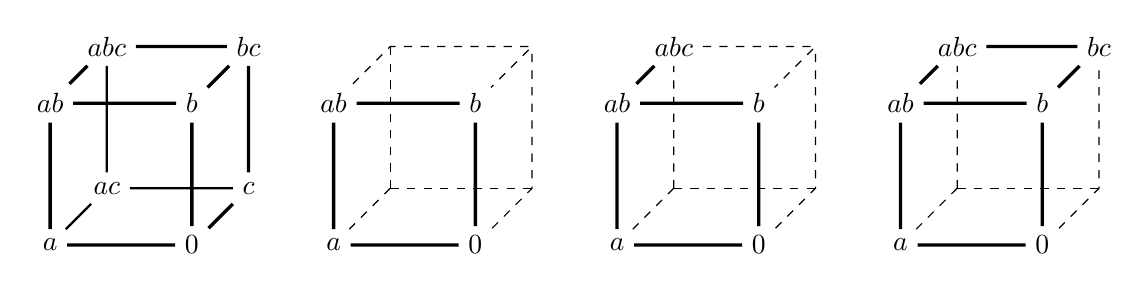
\begin{tikzpicture}[scale=1.8]
\begin{scope}[shift={(0,0)},local bounding box=aa]
    \node (0) at (0, 0) {$0$};
    \node (A) at (-1, 0) {$a$};
    \node (AB) at (-1, 1) {$ab$};
    \node (B) at (0, 1) {$b$};
    \node (C) at (0.4, 0.4) {$c$};
    \node (ABC) at (-0.6, 1.4) {$abc$};
    \node (BC) at (0.4, 1.4) {$bc$};
    \node (AC) at (-0.6, 0.4) {$ac$};

    \draw[very thick] (0) -- (A) -- (AB) -- (B) -- (0) ;
    \draw[very thick] (AB) -- (ABC) -- (BC) -- (B);
    \draw[very thick] (0) -- (C) -- (BC);

    \draw[thick] (AC) -- (A);
    \draw[thick] (AC) -- (ABC);
    \draw[thick] (AC) -- (C);        
\end{scope}

\begin{scope}[shift={(2,0)},local bounding box=bb]
    \node (0) at (0, 0) {$0$};
    \node (A) at (-1, 0) {$a$};
    \node (AB) at (-1, 1) {$ab$};
    \node (B) at (0, 1) {$b$};
    \coordinate (C) at (0.4, 0.4) {}; %{$c$};
    \coordinate (ABC) at (-0.6, 1.4) {}; % {$abc$};
    \coordinate (BC) at (0.4, 1.4) {}; % {$bc$};
    \coordinate (AC) at (-0.6, 0.4) {}; % {$ac$};

    \draw[very thick] (0) -- (A) -- (AB) -- (B) -- (0) ;
    \draw[dashed] (AB) -- (ABC) -- (BC) -- (B);
    \draw[dashed] (0) -- (C) -- (BC);

    \draw[dashed] (AC) -- (A);
    \draw[dashed] (AC) -- (ABC);
    \draw[dashed] (AC) -- (C);        
\end{scope}

\begin{scope}[shift={(4,0)},local bounding box=cc]
    \node (0) at (0, 0) {$0$};
    \node (A) at (-1, 0) {$a$};
    \node (AB) at (-1, 1) {$ab$};
    \node (B) at (0, 1) {$b$};
    \coordinate (C) at (0.4, 0.4) {};% {$c$};%
    \node (ABC) at (-0.6, 1.4) {$abc$};
    \coordinate (BC) at (0.4, 1.4) {};% {$bc$};%
    \coordinate (AC) at (-0.6, 0.4) {};% {$ac$};%

    \draw[very thick] (0) -- (A) -- (AB) -- (B) -- (0) ;
    \draw[very thick] (AB) -- (ABC);
    \draw[dashed] (ABC) -- (BC) -- (B);
    \draw[dashed] (0) -- (C) -- (BC);

    \draw[dashed] (AC) -- (A);
    \draw[dashed] (AC) -- (ABC);
    \draw[dashed] (AC) -- (C);        
\end{scope}

\begin{scope}[shift={(6,0)},local bounding box=dd]
    \node (0) at (0, 0) {$0$};
    \node (A) at (-1, 0) {$a$};
    \node (AB) at (-1, 1) {$ab$};
    \node (B) at (0, 1) {$b$};
    \coordinate (C) at (0.4, 0.4) {};% {$c$};%
    \node (ABC) at (-0.6, 1.4) {$abc$};
    \node (BC) at (0.4, 1.4) {$bc$};
    \coordinate (AC) at (-0.6, 0.4) {};% {$ac$};%

    \draw[very thick] (0) -- (A) -- (AB) -- (B) -- (0) ;
    \draw[very thick] (AB) -- (ABC) -- (BC) -- (B);
    \draw[dashed] (0) -- (C) -- (BC);

    \draw[dashed] (AC) -- (A);
    \draw[dashed] (AC) -- (ABC);
    \draw[dashed] (AC) -- (C);        
\end{scope}
\end{tikzpicture}
\caption{The Boolean lattice on 8 elements represented as a cube, and the 3 Heyting algebras of Figure \ref{fig:3HeytingAlgebras} embedded in this cube.}\label{fig:HAlgsInCubes}
\end{figure}

This hypercube representation immediately tells us that the Hasse diagrams of finite Heyting algebras are made up of lines and squares, and that no two squares can share more than one edge.  Figure \ref{fig:MoreHeytingAlgebras} illustrates a few more proper Heyting algebras, to give a sense of the range of shapes they can take.

\begin{figure}[htbp]
\centering
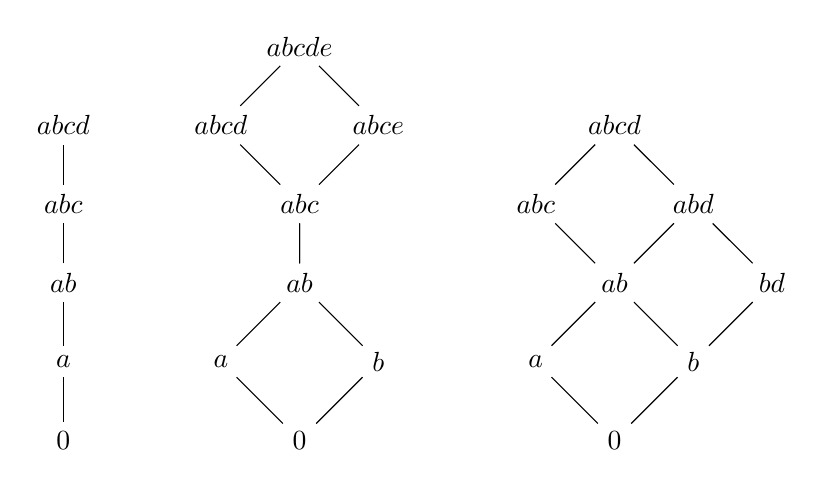
\begin{tikzpicture}[scale=.5]
\begin{scope}[shift={(0,0)},local bounding box=aa]
  \node (ABCD) at (0,8) {$abcd$};
  \node (ABC) at (0,6) {$abc$};
  \node (AB) at (0,4) {$ab$};
  \node (A) at (0,2) {$a$};
  \node (0) at (0,0) {$0$};
  
  \draw (0) -- (A)  -- (AB) -- (ABC) -- (ABCD); 
\end{scope}

\begin{scope}[shift={(6,0)},local bounding box=bb]
  \node (ABCDE) at (0,10) {$abcde$};
  \node (ABCD) at (-2,8) {$abcd$};
  \node (ABCE) at (2,8) {$abce$};
  \node (ABC) at (0,6) {$abc$};

  \node (AB) at (0,4) {$ab$};
  \node (A) at (-2,2) {$a$};
  \node (B) at (2,2) {$b$};
  \node (0) at (0,0) {$0$};
  
  \draw (0) -- (A)  -- (AB) -- (ABC) -- (ABCD) -- (ABCDE); 
  \draw (0) -- (B) -- (AB) -- (ABC) -- (ABCE) -- (ABCDE);
\end{scope}

\begin{scope}[shift={(14,0)},local bounding box=cc]
  \node (ABCD) at (0,8) {$abcd$};
  \node (ABC) at (-2,6) {$abc$};
  \node (ABD) at (2,6) {$abd$};
%  \node (AC) at (-4,4) {$ac$};
  \node (AB) at (0,4) {$ab$};
  \node (BD) at (4,4) {$bd$};
  \node (A) at (-2,2) {$a$};
  \node (B) at (2,2) {$b$};
  \node (0) at (0,0) {$0$};
  
  \draw (0) -- (A)  -- (AB) -- (ABC) -- (ABCD); 
  \draw (0) -- (B) -- (AB) -- (ABD) -- (ABCD);
%  \draw (A) -- (AC) -- (ABC);
  \draw (B) -- (BD) -- (ABD);
  \end{scope}



\end{tikzpicture}
\caption{Some more Heyting algebras.  Every chain forms a Heyting algebra (in which $\NOT x = 0$ for every element).  Heyting algebras can contain single edges between squares, as well as at the top and bottom.  Heyting algebras can be asymmetric.}\label{fig:MoreHeytingAlgebras}
\end{figure}



%\begin{table}[h]
%\centering
%\begin{tabular}{c|ccccc}
%$\IMPLIES$	& T & 2 & 3 & 4 & 0\\
%\hline
%T	&	T & 2 & 3 & 4 & 0	\\
%2	&	T & T & 3 & T & 3	\\
%3	&	T & 2 & T & T & 2	\\
%4	&	T & 2 & 3 & T & 0	\\
%0	&	T & T & T & T & T	\\
%\end{tabular}
%%
%\quad
%%
%\begin{tabular}{c|ccccc}
%$\AND$	& T & 2 & 3 & 4 & 0\\
%\hline
%T	&	T & 2 & 3 & 4 & 0	\\
%2	&	2 & 2 & 0 & 2 & 0	\\
%3	&	3 & 0 & 3 & 3 & 0	\\
%4	&	4 & 2 & 3 & 4 & 0	\\
%0	&	0 & 0 & 0 & 0 & 0	\\
%\end{tabular}
%%
%\quad
%%
%\begin{tabular}{c|ccccc}
%$\OR$	& T & 2 & 3 & 4 & 0\\
%\hline
%T	&	T & T & T & T & T	\\
%2	&	T & 2 & 4 & 4 & 2	\\
%3	&	T & 4 & 3 & 4 & 3	\\
%4	&	T & 4 & 4 & 4 & 4	\\
%0	&	T & 2 & 3 & 3 & 0	\\
%\end{tabular}
%\end{table} 




\subsection{Heyting algebras from preorders}

Another way to specify a Heyting algebra, which will be important in a later section, is to derive it as the lattice of upward closed sets of a preorder.  Let's unpack these terms.

A \terminology{preorder} is a binary relation on a set that is both reflexive and transitive, but need not be symmetric or antisymmetric.  We usually write the relation as $\leq$.

A subset $S$ of a preorder $(W, \leq)$ is \terminology{upward closed} 
if $x \in S$ and $x \leq y$ implies $y \in S$.  That is, if $S$ contains $x$ then it also contains every element of $W$ ``above'' $x$ in the preordering.  We will call an upward closed sets \emph{upsets} for short.  We will write $\uparrow x$ for the set of elements above $x$, i.e. $\uparrow x \DefinedAs \setSuchThat{y}{x \leq y}$, and we will call this the \emph{principal upset on $x$}.  An arbitrary upset is then a union of principal upsets.\footnote{
Trivially, the upset $S$ is the union $\bigcup_{s \in S} \uparrow S$, but there may be a smaller subset of $S$ that also serves as a base in this way (and a finite upset will always have a proper subset that serves as base).
}

Since upsets of $W$ are subsets of $W$, we can order them by subset inclusion.  We will now prove that this ordering on upsets makes then into a Heyting algebra.

\begin{Theorem}
The set of upsets on any preorder $(W, \leq)$, ordered by inclusion, form a Heyting algebra.
\end{Theorem}
\begin{Proof}
Let $(W, \leq)$ be a preorder.  We need to prove that the upsets of $(W, \leq)$ are closed under intersection and union, thus forming a lattice; that this lattice is bounded; and that we can define the $\to$ operation on lattice elements.  %
\begin{enumerate}[(a)]
\item If $P$ and $Q$ are upsets then for any element $i \in W$, 
\[
i \in P \intersect Q 
\iff
i \in P \mbox{ and } i \in Q
\]
Thus for any $j \geq i$, we have $j \in P$ and $i \in Q$, since $P$ and $Q$ are upsets, and thus $j \in P \intersect Q$.  Thus $P \intersect Q$ is also an upset.

\item If $P$ and $Q$ are upsets then for any element $i \in W$, 
\[
i \in P \union Q 
\iff
i \in P \mbox{ or } i \in Q
\]
Thus for any $j \geq i$, we either have $j \in P$ or $i \in Q$, since $P$ and $Q$ are upsets; in either case, $j \in P \union Q$.  Thus $P \union Q$ is also an upset.

\item The whole set $W$ itself is upward closed, and contains every upset as a subset; thus $W$ is the maximal element in the lattice.

\item The empty set $\varnothing$ is (trivially) upward closed, and is contained in every upset as a subset; thus $\varnothing$ is the minimal element in the lattice.

\item For upsets $P$ and $Q$, let 
\[
P \to Q
\DefinedAs
\setSuchThat{i \in W}{\uparrow i \subseteq \bar{P} \union Q}
\]
where $\bar{P} = W\setminus P$.  We will now prove that this satisfies the definition of $\to$ for a Heyting algebra, i.e. that it is the maximal upset $S$ such that $P \intersect S \subseteq Q$.
\begin{enumerate}[(i)]
\item First, $P \to Q$ is an upset: if 
$i \in P \to Q$ then $\uparrow i \subseteq \bar{P} \union Q$, and so for any $j \geq i$ we have ${\uparrow j} \subseteq {\uparrow i} \subseteq \bar{P} \union Q$, and thus $j \in P \to Q$.
%
\item Next, we prove that $P \intersect (P \to Q) \subseteq Q$.  Let 
$i \in P \intersect (P \to Q)$, so 
$\uparrow i \subseteq \bar{P} \union Q$, and so
$i \in \bar{P} \union Q$ (since the preorder relation is reflexive).  Thus 
\[
i \in (\bar{P} \union Q) \intersect P
= (\bar{P} \intersect P) \union (Q \intersect P)
= (Q \intersect P)
\]
by distributivity and the definition of $\bar{P}$.  Thus any $i$ in $P \intersect (P \to Q)$ is also in $Q$.
%
\item Finally, we prove that $P \to Q$ is the maximal such upset.  Let $X$ be an upset satisfying $X \intersect P \subseteq Q$.  Then we need to prove $X \subseteq (P \to Q)$.  Since $X$ is an upset, for any $x \in X$ we have $\uparrow x \subseteq X$.  But 
\[
X \intersect P \subseteq Q 
\iff
X \intersect P \intersect \bar{Q} = \varnothing
\iff
X \subseteq \bar{P} \intersect Q
\]
and so for any $x \in X$, $\uparrow x \subseteq X \subseteq \bar{P} \intersect Q$, and thus $x \in P \to Q$.
\end{enumerate}
\end{enumerate}
\end{Proof}

This gives us a useful way of constructing Heyting algebras -- we just give a preorder on some set and then order its upsets by subset inclusion.  As we'll see later, we can use this when we want to build Heyting algebra models of constructive logic satisfying certain properties.



\subsection{Logic with Heyting algebras}

Just as Boolean algebras provide the appropriate truth values for classical logic, Heyting algebras provide the appropriate truth values for constructive logic.


In Section \ref{sec:Models-TruthTables} we built a truth table for a formula in which each row corresponded to a way of assigning to each variable a truth value in the Boolean algebra $\{T, F\}$.  We can do exactly the same thing if we replace that Boolean algebra with any Heyting algebra -- since the usual logical operations are defined on a Heyting algebra, any assignment of values to the variables leads to a unique value for the formula itself.

We said that a formula is provable in CPL iff it is true under any assignment into $\{T, F\}$.  What is the corresponding result for constructive logic?  Which Heyting algebra plays the same role?  Unfortunately there is \emph{no} single Heyting algebra that serves the purpose.\footnote{As G\"{o}del proved in (1932).}  
However, what is true is that a formula is provable in constructive propositional logic iff it is a tautology -- i.e. gets the maximal value -- in \emph{every} Heyting algebra.  That means that if there is any assignment of values in any Heyting algebra that results in the formula getting a non-maximal value, then that formula is not provable constructively.  Thus we can still use truth tables to find  counterexamples to constructively invalid formulae.

As an example, consider again the formula 
$\NOT (P \AND Q) \IMPLIES ((\NOT P) \OR (\NOT Q))$.  We can evaluate this in any Heyting algebra, of course, but some will be more useful than others.  If we choose a Boolean algebra the formula will always get maximal value.  Likewise if we evaluate it in the 3-element chain.  But  in the 5-element Heyting algebra illustrated in Figure \ref{fig:3HeytingAlgebras} we can get a counterexample.  Since there are two variables we have $5^2=25$ rows to calculate, so we won't display the whole table -- but we don't need to.  To show that this formula is not constructively valid we just need to exhibit a single counterexample, i.e. a single row in which the formula does not have the maximal value $abc$ in that Heyting algebra, such as:
\begin{table}[h]
\centering
\begin{tabular}{c c|c c c}
P &	Q & $\NOT(P \AND Q)$ &	$(\NOT P) \OR (\NOT Q)$ &	$\NOT (P \AND Q) \IMPLIES ((\NOT P) \OR (\NOT Q))$ \\
\hline
a & b & 1 & ab & ab
\end{tabular}
\end{table}\\
That this is in fact a counterexample is easy to verify -- we simply have to evaluate the formula with the given values for the variables.  A Heyting algebra counterexample therefore provides a simple, compact, and easily verified demonstration that a given formula is not a tautology of constructive logic (and thus, via the Deduction theorem, that a given argument is not constructively valid).



\subsection{Building specific Heyting algebra counterexamples}

Although they are easy to verify, Heyting algebra counterexamples may not be easy to find.  For one thing, we do not know in advance \emph{which} Heyting algebra to evaluate into.  Then for any Heyting algebra we need to work out the entire truth table, which is a mechanical but tedious process.  It would be better, then, to have some means of producing counterexamples from formulae directly, or of demonstrating directly when a formula does not have a counterexample.

Ideally, what we would like (assuming we knew what Heyting algebra we should work in) is to construct a counterexample \emph{backwards}: starting with a non-maximal value in the right-most column of the truth table, we could then work from right to left, filling in the values that the preceding columns must take, until we eventually get to the left-most column containing the values of the variables.  


Of course, there are many factors that complicate matters.  First, we don't know which Heyting algebra we should be working in, and we don't yet even have a principle bounding the size of the Heyting algebras we need to consider.  Second, we don't know which non-maximal value the formula should take.  (For that matter, we don't even know in advance whether the formula has a counterexample at all -- that's what this process is supposed to find out.)  Then, for any given value in one column, there may be multiple compatible values that we could put in the preceding columns: for example, in two-valued Boolean logic, if we put $T$ in a column headed $A \OR B$ then there are 3 possible pairs of values we could assign to $A$ and $B$ that are compatible with this.  We would therefore need a \emph{branching} process, exploring each of these possibilities in parallel.

These various obstacles appear to make such a ``reverse-engineering'' of a counterexample unfeasible (or perhaps no less work than simply working out the whole truth table for a few Heyting algebras and hoping for some principle to guide us to the right one).  
However, a process based upon essentially this idea
 -- although with some major alterations! -- can be made to work, and this is the procedure we'll describe in the remainder of this section.

Rather than choosing the Heyting algebra in advance we will build it up indirectly by constructing a preorder by following certain rules depending upon the structure of the formula we are trying to disprove.  At the end of the procedure we will either have such a preorder, from which we can then obtain a Heyting algebra via the procedure of Section \ref{}, or we will find that no such preorder can be constructed.  In the latter case we wil have shown that there are no counterexamples to the formula, and thus the formula is a constructive tautology (and we should therefore direct our efforts into finding a constructive proof for it instead!)


\subsection{The rules of countermodel construction}

We want to define a preorder, so that we can obtain a Heyting algebra from it as its collection of upsets.  We also want to obtain an evaluation function from propositional variables and formulae into the Heyting algebra.  In particular, we want this evaluation to give a non-maximal value to the formula for which we are trying to give a countermodel.  So now we need to define a set of rules that will produce such a preorder for any formula that has a countermodel (i.e. any formula that is not a tautology of constructive logic).

If values in the Heyting algebra correspond to upsets in the preorder, then the valuation into the Heyting algebra, $h: F \to H$ should come from a valuation $\omega$ into the upsets of the preorder.  That is, for each formula $A$, $\omega(A)$ is an upward closed subset of the preorder.  It will also be useful to have a name for the complement of $\omega(A)$ in $W$, which we will denote $\bar{\omega}(A)$.


The valuation $h$ into the Heyting algebra that we obtain must be internally consistent -- for example, for any conjunction $A \AND B$ we must have $h(A \AND B) = h(A) \glb h(B)$.  If we pick values of $\omega$ arbitrarily then of course we can't expect this to hold, so we must impose rules on $\omega$ to guarantee consistency among values.  Specifically, we've seen in Section \ref{HAlgs-from-preorders} how the values must relate to one another: for all formulae $A$ and $B$,
\begin{itemize}
\item $\omega(A \AND B) \DefinedAs \omega(A) \intersect \omega{B}$
\item $\omega(A \OR B) \DefinedAs \omega(A) \union \omega{B}$
\item $\omega(A \to B) \DefinedAs 
\setSuchThat{i \in W}{\uparrow i \subseteq \bar{\omega}(A) \union \omega(B)}$
\end{itemize}
(where the latter condition follows from the fact that the upset corresponding to $A \to B$ must be the maximal upset $S$ such that $\omega(A) \intersect S \subseteq \omega(B)$.)

As usual, we define $\NOT A$ as $A \to \ABSURDITY$, where $\ABSURDITY$ is a contradictory proposition that is never true -- i.e. $\omega(\ABSURDITY) = \varnothing$.  Thus
\begin{itemize}
\item $\omega(\NOT A) \DefinedAs 
\setSuchThat{i \in W}{\uparrow i \subseteq \bar{\omega}(A)}$
\end{itemize}
Note that $\omega(\NOT A)$ is in general \emph{not} equal to $\bar{\omega}(A)$, but is always a subset of it.\footnote{
Proof sketch: if $i \in \omega(\NOT A)$ then $\uparrow i \subseteq \bar{\omega}(A)$, and we always have $i \in \uparrow i$, so 
$i \in \omega(\NOT A) \subseteq \bar{\omega}(A)$.  But for the converse dirction, $j \in \bar{\omega}(A)$ is not sufficient to guarantee $\uparrow j \subseteq \bar{\omega}(A)$, so in general $j \not\in \omega(\NOT A)$ and thus $\bar{\omega}(A) \not\subseteq \omega(\NOT A)$.
}
That is, $\omega(\NOT A) \intersect \omega(A) = \varnothing$, but 
$\omega(\NOT A) \union \omega(A) \neq W$, as we would expect for an intuitionistic logic.

We noted above that the whole preorder, being an upset, serves as the maximal element $1$ of the Heyting algebra.  Thus if the preorder has a root element -- i.e. a world $w_0$ such that $\forall w \in W,\, w_0 \leq w$ -- then any formula $A$ with $w_0 \in \omega(A)$ must (by the requirement that $\omega(A)$ be an upset) have $\omega(A) = W$, and therefore gets value $1$ in the Heyting algebra.  Conversely, to ensure that a formula $A$ does \emph{not} get maximal value in the Heyting algebra, we just need to ensure that $w_0 \not\in \omega(A)$.  This therefore gives our final two conditions when building a counterexample to $A$: ensure that the preorder has a root world $w_0$, and set $w_0 \not\in \omega(A)$.


So, given a formula $\phi$ that we wish to show is not a tautology, we  need to construct a rooted preorder $(W, \leq, w_0)$ and an evaluation function $\omega: F \to 2^W$ that assigns to each formula\footnote{
Specifically, to each formula using the same propositional variables as $\phi$.} 
an upward-closed subset of $W$, ensuring that $\omega$ obeys the rules above, and in which $w_0 \not\in \omega(\phi)$.  In the next section we will see the procedure that allows us to carry out this construction if it it possible.



%Another way to encode the same information is via a function $\nu: W \times F \to \set{0,1}$, defined by
%\[
%\nu(i, A) = 1 \quad \iff \quad i \in \omega(A)
%\]
%To ensure that the sets of worlds assigned to each formula are upward closed, we must impose a condition: if $\nu(i,A) = 1$ then for all $j \geq i$ in the preorder, $\nu(j,A) = 1$.

%For $\AND$ and $\OR$ the rules are obvious: for all $i \in W$, and all formulae $A$ and $B$,
%\[
%\nu(i,A \AND B) = 1 \quad \mbox{ iff } \quad 
%\nu(i,A) = 1 \mbox{ and } \nu(i,B) = 1
%\]
%\[
%\nu(i,A \OR B) = 1 \quad \mbox{ iff } \quad 
%\nu(i,A) = 1 \mbox{ or } \nu(i,B) = 1
%\]
%Equivalently, we can express these as sums and products of values:
%\begin{align*}
%\nu(i,A \AND B) &\DefinedAs 
%\nu(i,A) \times \nu(i,B)
%\\
%\nu(i,A \OR B) &\DefinedAs
%\nu(i,A) + \nu(i,B) - \nu(i,A) \times \nu(i,B)
%\end{align*}





%Part of the problem here is that when we do constructive logic all we know at a given time is which types we have terms for -- we have no way of positively recording the fact that we \emph{don't} have a term of a given type.  The mere omission of a term from the list of things we're given is not sufficient, since it may be possible to construct such a term from the things we are given and we have simply not yet done so.  That is, the fact that a term has not been constructed in a given context is not evidence that it \emph{cannot} be constructed in that context.  But it is precisely the latter that we need to demonstrate in order to show that a particular construction is not possible.  We therefore need a new approach to studying constructive arguments, in which both the presence and absence of terms can be actively recorded.
%
%In a constructive model, the failure to record that a term is present does not correspond to that term's being absent.  We models we require must therefore be \emph{classical}.  
%
%
%\subsubsection{Definition of Kripke models}
%
%A \terminology{Kripke frame} is a pair of a non-empty set $W$, whose elements we call \terminology{worlds}, and a binary relation $R$ on $W$, which we call \terminology{accessibility}.  For the most general Kripke frame we assume no particular properties of $R$.  However, for present purposes we will restrict attention to Kripke frames whose accessibility relations are \emph{reflexive} and \emph{transitive} (i.e. which are \emph{preorders}).  We therefore write the accessibility relation as $\leq$.
%
%An \terminology{intuitionistic Kripke model} is then a Kripke frame along with a relation $\makestrue$ between worlds and expressions of our language, such that:
%\begin{samepage}
%\begin{itemize}
%\item $w \makestrue A \AND B$ iff $w \makestrue A$ and $w \makestrue B$
%\item $w \makestrue A \OR B$  iff $w \makestrue A$ or  $w \makestrue B$
%\item $w \makestrue A \IMPLIES B$ iff for all $u \geq w$, $u \makestrue A$ implies $u \makestrue B$
%\item $w \not \makestrue \ABSURDITY$
%\item for any propositional variable, if $w \makestrue p$ and $w \leq u$ then $u \makestrue p$
%\end{itemize}
%\end{samepage}
%










